\documentclass[11pt,a4paper,final]{article} %draft

\usepackage[T1,T2A]{fontenc}
\usepackage[utf8]{inputenc}
\usepackage[english, russian]{babel}

\usepackage[final]{pdfpages}

\usepackage{textcomp,enumitem}

\usepackage{amsmath,amsthm,amssymb}

\usepackage{fancyhdr} % для настройки страницы и колонтитулов

\usepackage{graphicx}

\usepackage{indentfirst} % автоматический отступ в начале каждого раздела

\usepackage[unicode, pdftex, colorlinks, urlcolor=blue]{hyperref}

\usepackage[left=2cm,right=2cm,top=2cm,bottom=2cm,bindingo ffset=0cm]{geometry}

\linespread{1.3} % устанавливает междустрочный интервал

\pagestyle{plain} % для отображения номеров внизу 

\usepackage{float}

\usepackage{listings} 

\usepackage{pdflscape}
\usepackage{listings} 
\definecolor{darkgreen}{rgb}{0,0.5,0}

\lstset{
	backgroundcolor=\color{white},  % Устанавливаем белый фон для блока кода
	basicstyle=\ttfamily\small\fontfamily{inconsolata}\selectfont,  % Основной стиль текста: моноширинный шрифт Inconsolata с небольшим размером
	commentstyle=\color{darkgreen}\slshape,  % Комментарии будут зелеными и курсивными
	keywordstyle=\color{blue}\bfseries,  % Ключевые слова выделяются синим цветом и полужирным шрифтом
	numberstyle=\scriptsize\color{gray},  % Стиль нумерации строк: маленький размер шрифта и серый цвет
	stringstyle=\color{orange},  % Строки (текст в кавычках) отображаются оранжевым цветом
	breakatwhitespace=false,  % Не прерывать строки только по пробелам
	breaklines=true,  % Автоматический перенос длинных строк
	captionpos=b,  % Позиция заголовка/описания для блока кода — внизу (b — bottom)
	keepspaces=true,  % Сохранить пробелы, как они есть, в исходном коде
	numbers=left,  % Нумерация строк будет отображаться слева
	numbersep=5pt,  % Отступ между строками кода и номерами строк (4pt)
	showspaces=false,  % Не показывать пробелы
	showstringspaces=false,  % Не показывать пробелы внутри строк
	showtabs=false,  % Не показывать символы табуляции
	tabsize=4,  % Размер табуляции — 4 пробела
	language=c++,  % Указываем язык программирования для синтаксического подсветки (C++)
	captionpos=t,  % Заголовок кода будет размещен вверху (t — top)
	xleftmargin=0mm,  % Убираем отступ слева
	frame=single,  % Однотонная рамка вокруг блока кода
	framerule=0.25mm,  % Толщина рамки — 0.25 мм
	literate=
	{а}{{\selectfont\char224}}1
	{б}{{\selectfont\char225}}1
	{в}{{\selectfont\char226}}1
	{г}{{\selectfont\char227}}1
	{д}{{\selectfont\char228}}1
	{е}{{\selectfont\char229}}1
	{ж}{{\selectfont\char230}}1
	{з}{{\selectfont\char231}}1
	{и}{{\selectfont\char232}}1
	{й}{{\selectfont\char233}}1
	{к}{{\selectfont\char234}}1
	{л}{{\selectfont\char235}}1
	{м}{{\selectfont\char236}}1
	{н}{{\selectfont\char237}}1
	{о}{{\selectfont\char238}}1
	{п}{{\selectfont\char239}}1
	{р}{{\selectfont\char240}}1
	{с}{{\selectfont\char241}}1
	{т}{{\selectfont\char242}}1
	{у}{{\selectfont\char243}}1
	{ф}{{\selectfont\char244}}1
	{х}{{\selectfont\char245}}1
	{ц}{{\selectfont\char246}}1
	{ч}{{\selectfont\char247}}1
	{ш}{{\selectfont\char248}}1
	{щ}{{\selectfont\char249}}1
	{ъ}{{\selectfont\char250}}1
	{ы}{{\selectfont\char251}}1
	{ь}{{\selectfont\char252}}1
	{э}{{\selectfont\char253}}1
	{ю}{{\selectfont\char254}}1
	{я}{{\selectfont\char255}}1
	{А}{{\selectfont\char192}}1
	{Б}{{\selectfont\char193}}1
	{В}{{\selectfont\char194}}1
	{Г}{{\selectfont\char195}}1
	{Д}{{\selectfont\char196}}1
	{Е}{{\selectfont\char197}}1
	{Ж}{{\selectfont\char198}}1
	{З}{{\selectfont\char199}}1
	{И}{{\selectfont\char200}}1
	{Й}{{\selectfont\char201}}1
	{К}{{\selectfont\char202}}1
	{Л}{{\selectfont\char203}}1
	{М}{{\selectfont\char204}}1
	{Н}{{\selectfont\char205}}1
	{О}{{\selectfont\char206}}1
	{П}{{\selectfont\char207}}1
	{Р}{{\selectfont\char208}}1
	{С}{{\selectfont\char209}}1
	{Т}{{\selectfont\char210}}1
	{У}{{\selectfont\char211}}1
	{Ф}{{\selectfont\char212}}1
	{Х}{{\selectfont\char213}}1
	{Ц}{{\selectfont\char214}}1
	{Ч}{{\selectfont\char215}}1
	{Ш}{{\selectfont\char216}}1
	{Щ}{{\selectfont\char217}}1
	{Ъ}{{\selectfont\char218}}1
	{Ы}{{\selectfont\char219}}1
	{Ь}{{\selectfont\char220}}1
	{Э}{{\selectfont\char221}}1
	{Ю}{{\selectfont\char222}}1
	{Я}{{\selectfont\char223}}1,
	numbers=left, % пронумеровать строки с левой стороны
	breaklines=true % разрешает автоматический перенос строк
}

\hypersetup{
	colorlinks=true, % делает ссылки цветными вместо рамки
	linkcolor=blue, % цвет внутренних ссылок
	urlcolor=blue, % цвет внешних ссылок
	citecolor=blue % цвет ссылок на литературу в тексте
}
\textheight=24cm 
\textwidth=16cm
\oddsidemargin=0pt 
\topmargin=-1.5cm
\parindent=24pt 
\parskip=0pt 
\tolerance=2000 
\flushbottom 

%\usepackage[font=scriptsize]{caption}
\usepackage[labelsep=period]{caption}

\usepackage{amsmath}

\begin{document}

\thispagestyle{empty}

\begin{center}
	{\Large МИНОБРНАУКИ РОССИИ}\\
	~\\
	{\large ФЕДЕРАЛЬНОЕ ГОСУДАРСТВЕННОЕ БЮДЖЕТНОЕ ОБРАЗОВАТЕЛЬНОЕ УЧРЕЖДЕНИЕ ВЫСШЕГО ПРОФЕССИОНАЛЬНОГО ОБРАЗОВАНИЯ}\\
	~\\
	{\Large \bf <<САНКТ-ПЕТЕРБУРГСКИЙ ПОЛИТЕХНИЧЕСКИЙ УНИВЕРСИТЕТ ПЕТРА ВЕЛИКОГО>>}\\
	~\\
	{\large Институт компьютерных наук и кибербезопасности }\\
	{\large Высшая школа технологий искусственного интеллекта}\\
	{\large Направление 02.03.01 Математика и компьютерные науки}\\
	~\\
	~\\
	~\\
	~\\
	{\Large \bf  Отчет по лабораторной работе }\\
	\vspace{3mm}
	{\Large {по дисциплине <<Архитектура суперкомпьютеров>>}}\\
	\vspace{3mm}
	{\Large \bf Разработка приложения, моделирующего работу механизма передачи сообщения в коммуникационной сети суперкомпьютера. }\\
	~\\
	~\\
	~\\
	~\\
	~\\
	{\large Обучающийся: \underline{\hspace{3.5cm}} \hspace{12mm} Шихалев А.О.}\\
	~\\
	{\large Руководитель: \underline{\hspace{3.5cm}} \hspace{12mm} Чуватов М.В.}\\
	~\\
	~\\
	~\\
	~\\
\end{center}
\begin{flushright}
	
	«\underline{\hspace{1cm}}»\underline{\hspace{3cm}}20\underline{\hspace{0.7cm}}г.
\end{flushright}
~\\
~\\
\begin{center}
	{\large Санкт-Петербург, 2024}
\end{center}

\newpage

\tableofcontents

\newpage
\section* {Введение}
\addcontentsline{toc}{section}{Введение}

\par Отчет представляет собой описание выполненной лабораторной работы по дисциплине <<Архитектура суперкомпьютеров>>. Лабораторная работа включает в себя реализацию приложения, моделирующего работу механизма передачи сообщения в коммуникационной сети суперкомпьютера. В приложении реализована функция отправки сообщения, которая вызывается в формате (АДРЕС\_ИСТОЧНИКА ДЛИНА\_СООБЩЕНИЯ АДРЕС\_ПОЛУЧАТЕЛЯ) и которая включает в себя функцию вычисления маршрута передачи сообщения с целью минимизации времени, необходимого для передачи. ДЛИНА\_СООБЩЕНИЯ -- это число шагов, требуемых для его передачи по свободному каналу. Также реализована возможность продвигаться по шагам, и в начале каждого шага пользователь может указать от 0 до 10 заданий на пересылку сообщений с произвольными адресами источника и получателя. Важной особенностью является штраф за каждую пересылку через промежуточный узел или через коммутатор в 1 дополнительный шаг времени. В качестве использованной топологии была выбрана топология Dragonfly со следующими характеристиками:
\begin{itemize}
	\item Число групп: 13
	\item Коммутаторов в группе: 4
	\item Узлов на коммутатор: 3
	\item Пропускная способность внутри группы: 4
	\item Пропускная способность между группами: 3
\end{itemize}



\par Работа была выполнена в среде Visual Studio 2022 на языке программирования С++.	
	

\newpage
\section {Математическое описание}

\subsection {Коммуникационные сети суперкомпьютеров} 

\par Коммуникационные сети суперкомпьютеров — это критически важная часть архитектуры, которая обеспечивает связь между отдельными узлами (процессорами, серверами, вычислительными блоками) для выполнения параллельных вычислений. Эти сети должны быть чрезвычайно быстрыми и эффективными, чтобы минимизировать задержки и обеспечить максимальную пропускную способность для обмена данными.

\par Основные компоненты коммуникационной сети:

\begin{enumerate}
	\item \textbf{Узлы} — это вычислительные элементы (процессоры, ядра или серверы), которые обмениваются данными. Каждый узел имеет сетевые адаптеры, через которые они подключены к сети.
	\item \textbf{Коммутаторы} — это устройства, которые управляют потоком данных между узлами, перенаправляя данные от одного узла к другому по оптимальному пути.
	\item \textbf{Маршрутизация} — процесс определения путей передачи данных между узлами через коммутаторы. Эффективные алгоритмы маршрутизации играют ключевую роль в минимизации задержек.
	\item \textbf{Сетевые интерфейсы} — это интерфейсы, через которые узлы подключаются к сети (например, InfiniBand, Ethernet, или специализированные сети).
\end{enumerate}

\par Ключевые характеристики коммуникационных сетей:

\begin{itemize}
	\item \textbf{Пропускная способность} (Bandwidth) — максимальное количество данных, которое может передаваться по сети за единицу времени.
	\item \textbf{Задержка} (Latency) — время, которое требуется для передачи данных от одного узла к другому.
	\item \textbf{Прямое соединение} (Direct Connection) — возможность узлов обмениваться данными напрямую без участия коммутаторов.
	\item \textbf{Трафик} (Traffic Pattern) — типы передач данных, например, all-to-all (все ко всем), one-to-all (один ко всем), one-to-one (один к одному).
	\item \textbf{Отказоустойчивость} (Fault Tolerance) — сети суперкомпьютеров проектируются таким образом, чтобы справляться с отказами отдельных узлов или соединений без серьезного влияния на общую производительность.
\end{itemize}

\subsection{Сетевые топологии}

\par Сетевые топологии — это схема организации связи между узлами в вычислительной системе, такие как суперкомпьютеры, серверы или рабочие станции. Топология сети определяет, как данные передаются между узлами, насколько эффективно сеть масштабируется, и насколько быстро она обрабатывает запросы. Выбор топологии влияет на производительность, устойчивость к отказам и стоимость создания и поддержания сети.

\par Основные типы топологий сетей, используемых в сети суперкомпьютеров:

\begin{enumerate}
	\item \textbf{Полносвязная топология} -- каждый узел сети напрямую соединён со всеми другими узлами. Это минимизирует задержки при передаче данных, так как каждый узел может обмениваться данными без участия промежуточных узлов.
	
	\item \textbf{Fat-tree} (Толстое дерево) -- древовидная топология с высокой пропускной способностью на каждом уровне, благодаря расширенным (``жирным'') каналам между уровнями. У каждого уровня дерева есть более широкие каналы для соединения с более высоким уровнем. В этой топологии узлы на нижнем уровне связаны с узлами верхних уровней через несколько уровней коммутаторов.
	
	
	\item \textbf{Тор} представляет собой двумерную или трёхмерную сетку узлов, в которой каждый узел соединён с ближайшими соседями, а крайние узлы соединяются друг с другом, создавая ``кольцевую'' структуру. В трёхмерной версии каждый узел связан с соседями по трём направлениям (например, x, y, z).
	
	\item \textbf{Dragonfly} — это иерархическая сеть, где узлы объединены в группы, каждая из которых представляет собой почти полносвязную структуру. Между группами создаются ограниченные глобальные соединения, что снижает количество коммутаторов и кабелей, требуемых для межгрупповой связи.
	
	\item \textbf{Гиперкуб} — это топология, в которой каждый узел представляет вершину многомерного куба. В двумерной версии (2D) каждый узел соединён с двумя соседями, а в трёхмерной версии (3D) узлы соединены с тремя соседями. С увеличением измерений количество узлов и соединений растёт экспоненциально.
	
	\item \textbf{Butterfly} -- данные передаются через несколько уровней узлов, где каждый уровень имеет узлы, соединённые с узлами следующего уровня по заранее определённой схеме, напоминающей "крылья бабочки". Это позволяет эффективно распределять данные между узлами через минимальное количество уровней.
	
\end{enumerate}

\subsection{Топология Dragonfly}

Топология Dragonfly — это современная топология, разработанная для высокопроизводительных вычислительных систем, таких как суперкомпьютеры, с целью обеспечения высокой производительности при минимальных затратах на межузловую коммуникацию. Dragonfly сочетает идеи из <<Fat-tree>>, <<Torus>> и других топологий для создания эффективной, высокомасштабируемой сети.

\textbf{Основные черты Dragonfly:}
\begin{enumerate}
	
\item Иерархическая структура:

\begin{itemize} 
	\item Группы: Сеть разбита на группы, внутри которых узлы соединены полносвязно или почти полносвязно. Группы могут состоять из подгрупп узлов, связанных между собой с высокой пропускной способностью.
	\item Межгрупповые соединения: Узлы из разных групп соединены меньшим числом связей через специальные маршрутизаторы или коммутаторы, обеспечивая глобальные связи между группами.
\end{itemize}

\item Минимизация числа соединений: Каждая группа связана только с небольшим количеством других групп, что снижает общие требования к числу межгрупповых соединений и позволяет строить сети с тысячами или даже миллионами узлов.

\item Эффективное распределение нагрузки: Топология Dragonfly использует адаптивные алгоритмы маршрутизации, чтобы избежать перегрузок в межгрупповых каналах и сбалансировать нагрузку между узлами и группами.
\end{enumerate}


\textbf{Преимущества топологии Dragonfly:}
\begin{itemize}
\item Отличная масштабируемость: Топология поддерживает большие кластеры с тысячами узлов, при этом минимизируя количество межгрупповых соединений.
\item Высокая пропускная способность: Полносвязные группы и прямые соединения между группами обеспечивают высокую скорость передачи данных.
\item Снижение задержек: Адаптивная маршрутизация позволяет минимизировать задержки и сбалансировать нагрузку.
\end{itemize}

\par Структура топологии Dragonfly представлена на \hyperref[fig:pic1]{рисунке 1}.
\newpage
\begin{figure}[H]
	\centering
	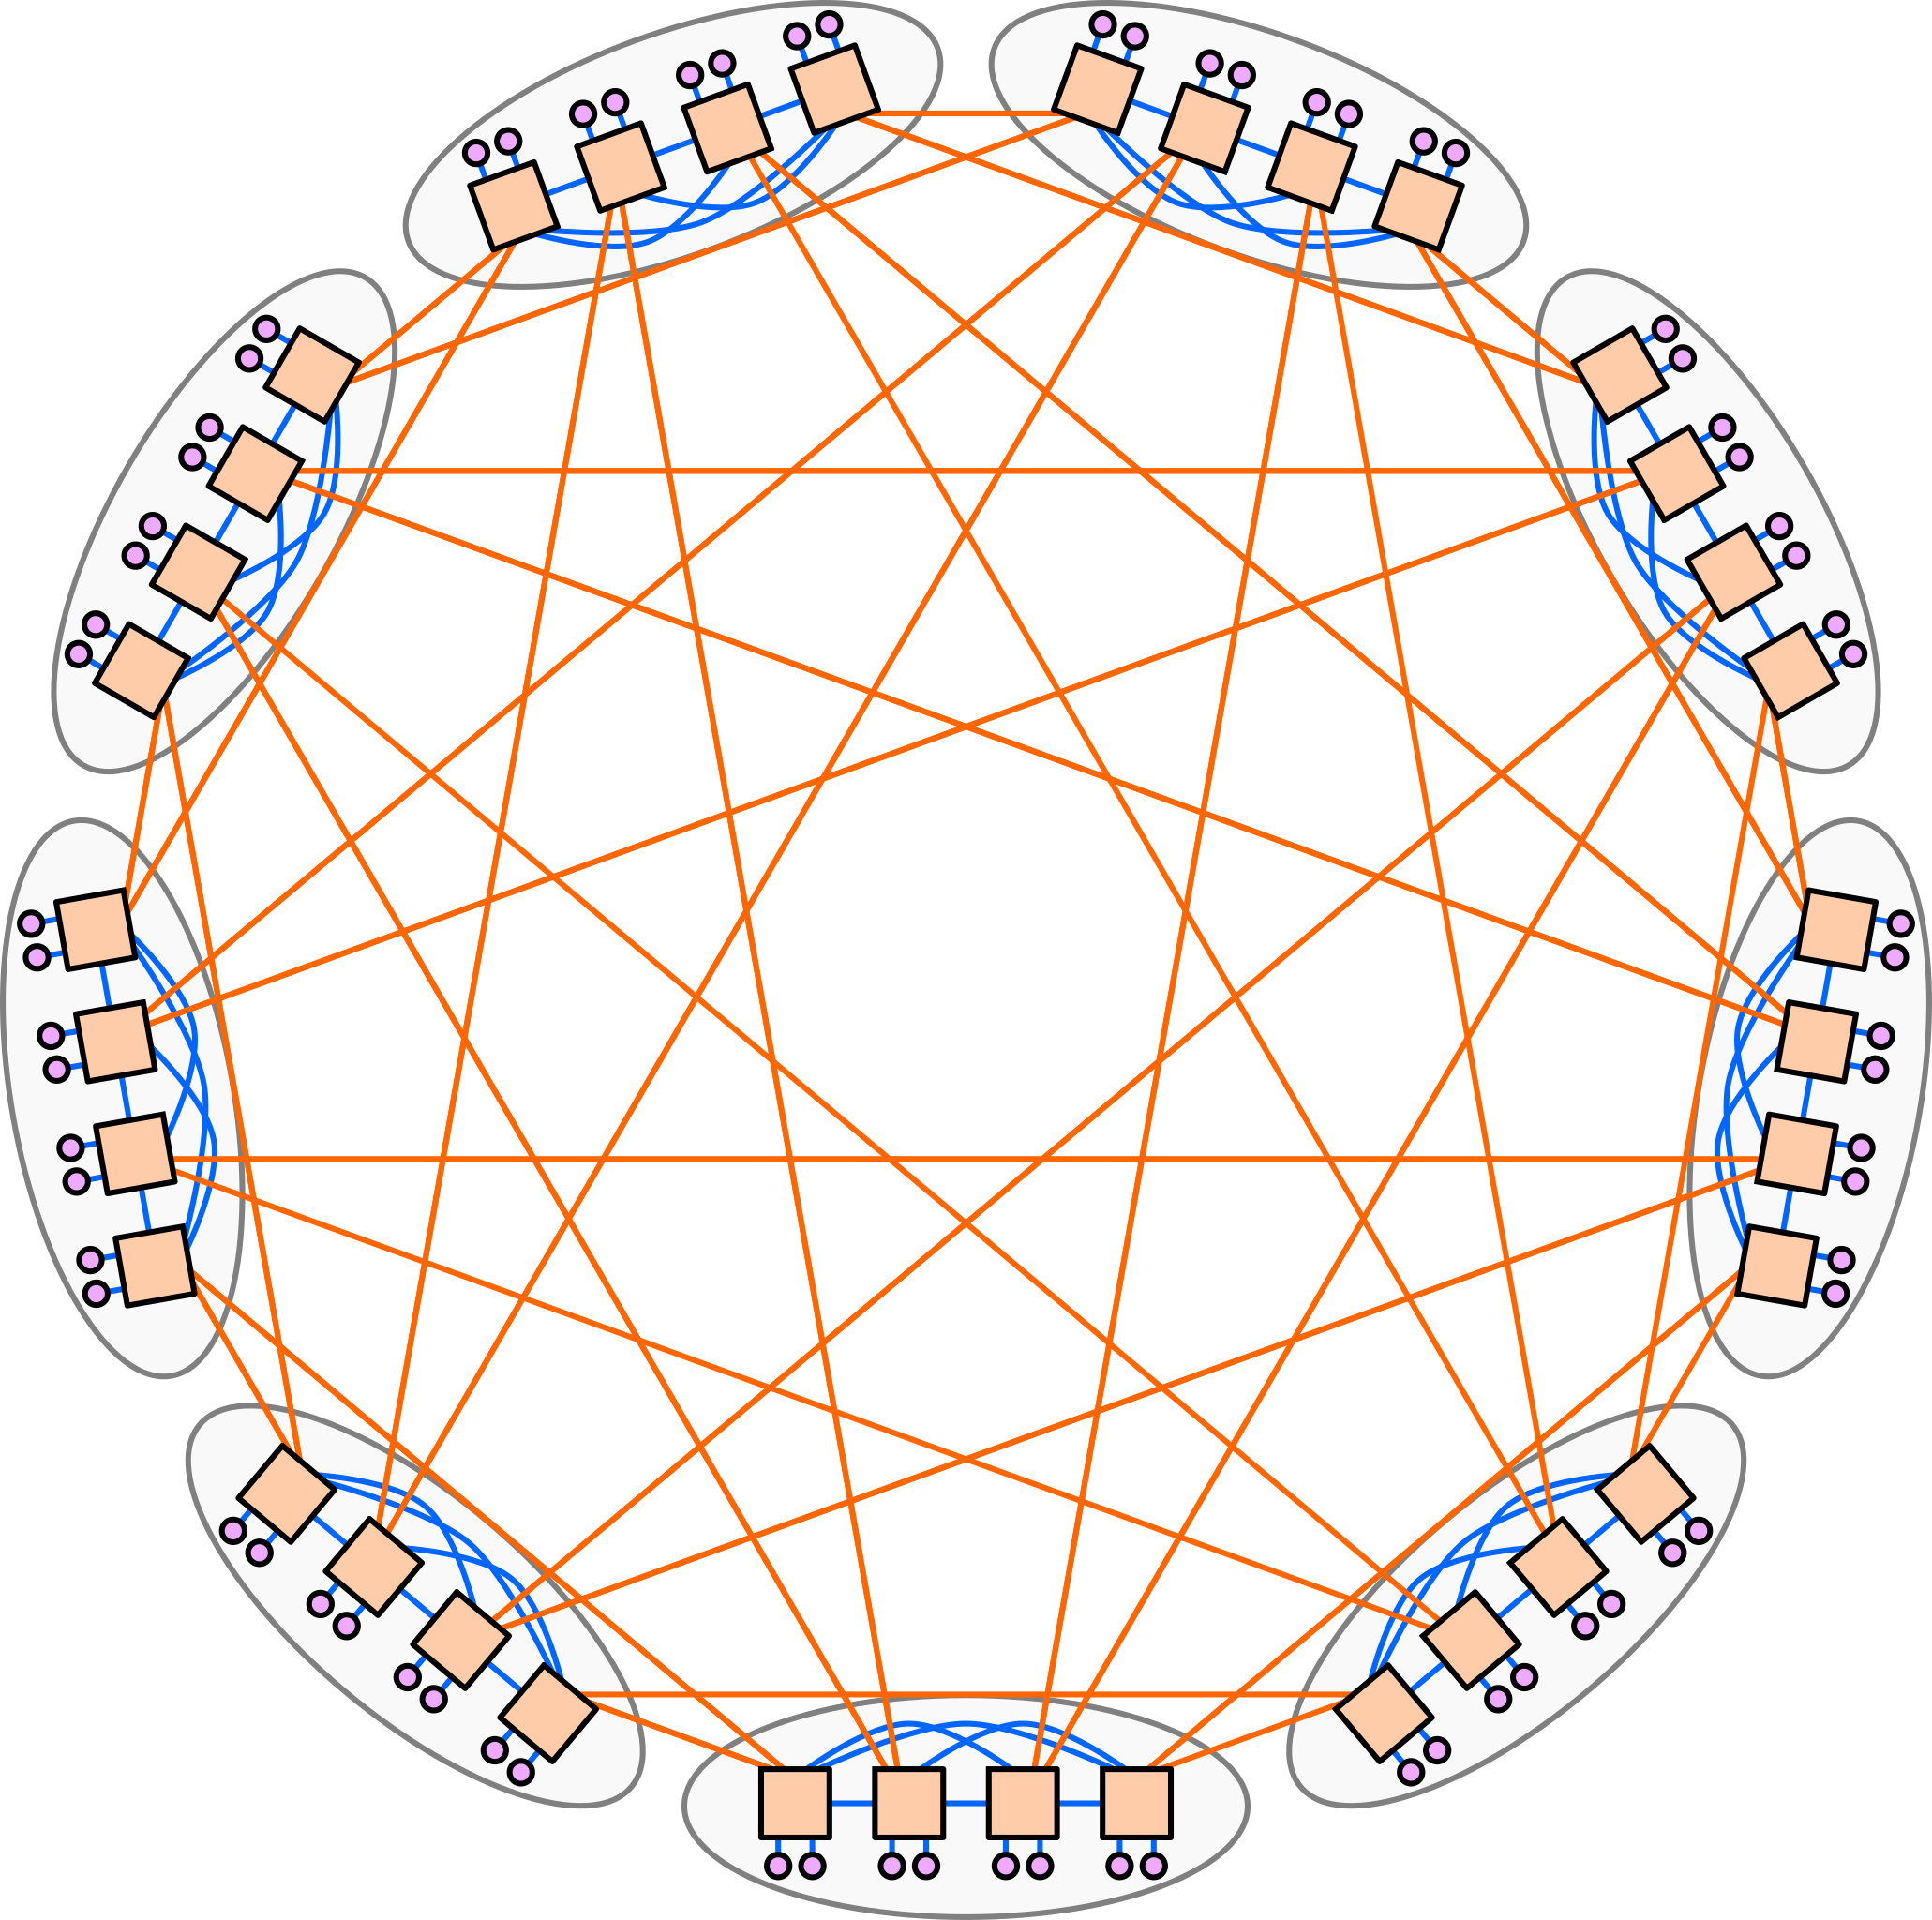
\includegraphics[width=0.8\linewidth]{pic1.png}
	\caption{Структура топологии Dragonfly}
	\label{fig:pic1}
\end{figure}





\newpage
\section{Особенности реализации}

\subsection{Класс Network}

\textbf{Класс \texttt{Network}} предназначен для моделирования сетевой структуры заданной в варианте топологии, состоящей из нескольких групп, коммутаторов и узлов. Основная цель класса — управление сетевыми ресурсами, такими как пропускная способность внутри группы и между группами, а также обработка сообщений в сети.

\textbf{Поля класса Network:}
\begin{itemize}
	\item \texttt{GROUPS} — количество групп в сети.
	\item \texttt{COMMUTATORS} — количество коммутаторов в каждой группе.
	\item \texttt{NODES} — количество узлов, подключенных к каждому коммутатору.
	\item \texttt{BANDWIDTH\_IN\_GROUP} — пропускная способность внутри группы.
	\item \texttt{BANDWIDTH\_BETWEEN\_GROUP} — пропускная способность между группами.
	\item \texttt{messages} — вектор, содержащий сообщения, обрабатываемые сетью.
	\item \texttt{status} — вектор строк, описывающих статус каждого сообщения.
	\item \texttt{path} — вектор векторов, содержащий пути передачи сообщений.
	\item \texttt{reserv} — вектор, описывающий количество зарезервированных ресурсов на каждом шаге передачи сообщения.
	\item \texttt{reminder} — вектор, содержащий информацию о том, сколько данных осталось передать между вершинами.
	\item \texttt{matrix\_bandwidth} — матрица пропускных способностей сети.
	\item \texttt{matrix\_load} — матрица загруженности сети.
\end{itemize}

\subsection{Конструктор класса Network}

Класс Network имеет параметризованный конструктор, который позволяет задать количество групп, коммутаторов, узлов, а также пропускную способность внутри группы и между группами. Помимо этого, он строит матрицу пропускных способностей и матрицу загруженности для заданной сети.

Реализация конструктора представлена в \hyperref[lst1]{листинге 1}.
\newpage
\begin{lstlisting}[label=lst1, caption = Конструктор класса Network]
Network::Network(int GROUPS, int COMMUTATORS, int NODES, int BANDWIDTH_IN_GROUP, int BANDWIDTH_BETWEEN_GROUP)  {
	this->GROUPS = GROUPS;
	this->COMMUTATORS = COMMUTATORS;
	this->NODES = NODES;
	this->BANDWIDTH_IN_GROUP = BANDWIDTH_IN_GROUP;
	this->BANDWIDTH_BETWEEN_GROUP = BANDWIDTH_BETWEEN_GROUP;
	
	count_commutators = GROUPS * COMMUTATORS; 
	count_nodes = count_commutators * NODES; 
	count_vertex = count_commutators + count_nodes;
	
	vector<vector<int>> new_bandwidth(count_vertex, vector<int>(count_vertex, 0));
	matrix_bandwidth = new_bandwidth;
	
	
	for (int i = 0, ii=count_nodes, k = NODES; i < count_nodes;i++) {
		k--;
		matrix_bandwidth[i][ii] = BANDWIDTH_IN_GROUP; //пропускная способность в группе
		matrix_bandwidth[ii][i] = BANDWIDTH_IN_GROUP;
		if (k == 0) {
			ii++;
			k = NODES;
		}	
	}
	
	
	for (int i = 0, back=COMMUTATORS-1, group=GROUPS-1; i < COMMUTATORS; i++, back--, group-=GROUPS/COMMUTATORS) {
		
		
		for (int ii = count_nodes + i, group_right=group ; ii < count_vertex; ii+=COMMUTATORS, group_right++) {
			if (group_right >= GROUPS) {
				group_right -= GROUPS;
			}
			for (int iii = 0, current_group = group_right; iii < GROUPS/COMMUTATORS; iii++) {
				current_group = (group_right - iii) < 0 ? GROUPS + (group_right - iii) : group_right - iii;
				int buf = count_nodes + current_group * COMMUTATORS + back; 
				matrix_bandwidth[ii][count_nodes + current_group * COMMUTATORS + back] = BANDWIDTH_BETWEEN_GROUP;//пропускная способность между группами
				matrix_bandwidth[count_nodes + current_group * COMMUTATORS + back][ii] = BANDWIDTH_BETWEEN_GROUP;
			}
		}
	}
	
	for (int i = 0; i < GROUPS; i++) {
		for (int ii = count_nodes + i * COMMUTATORS; ii < count_nodes + (i + 1) * COMMUTATORS; ii++) {
			for (int iii = ii; iii < count_nodes + (i + 1) * COMMUTATORS; iii++) {
				if (ii != iii) {
					matrix_bandwidth[ii][iii] = BANDWIDTH_IN_GROUP;//пропускная способность в группе
					matrix_bandwidth[iii][ii] = BANDWIDTH_IN_GROUP;
				}
			}
		}
	}
	
	matrix_load = matrix_bandwidth;
}
\end{lstlisting}

\subsection{Модифицированный алгоритм Дейкстры}

Метод \texttt{Dijkstra\_algorythm} реализует модифицированный алгоритм Дейкстры для поиска кратчайшего пути в сети с учетом загруженности соединений и штрафов за пересечение промежуточных узлов.

Метод принимает параметр \texttt{message} — вектор из трех элементов: \texttt{message[0]} — исходный узел, \texttt{message[1]} — длина сообщения, \texttt{message[2]} — конечный узел.

Реализация алгоритма представлена в \hyperref[lst2]{листинге 2}.

\begin{lstlisting}[label=lst2, caption = {Модифицированный алгоритм Дейкстры}]
vector<int> Network::Dijkstra_algorythm(vector<int> message) {
	int index_from = message[0];
	int index_to = message[2];
	int cost = message[1];
	
	int count = 0;
	vector<int> vertex(count_vertex);
	for (int i = 0; i < vertex.size(); i++) {
		vertex[i] =  INT_MAX;
	}
	vector<bool> vertex_check(count_vertex, false);
	vector<vector<int>> route(count_vertex);
	vertex[index_from] = 0;
	
	int current;
	while (CheckBoolVector(vertex_check) == false) {
		current = Min_Index(vertex, vertex_check, cost) ;
		if (current == -1)
		break;
		vertex_check[current] = true;
		
		for (int i = 0; i < matrix_load[current].size(); i++) {
			if (matrix_load[current][i] != 0) {
				int buf = cost / matrix_load[current][i];
				buf = cost % matrix_load[current][i]==0? buf :buf + 1;
				if (!(current == index_from || current == index_to)) {
					buf++; //прибавляем штраф
				}
				bool condition = vertex[current] + buf <= vertex[i];
				if (condition) {
					
					vertex_check[i] = false;
					route[i].clear();
					route[i] = route[current];
					route[i].push_back(current);
					vertex[i] = vertex[current] + buf;
				}
			}
		}
	}
	for (int i = 0; i < vertex.size(); i++) {
		if (vertex[i] == INT_MAX || vertex[i] == INT_MAX + 1)
		vertex[i] = 0;
	}
	for (int i = 0; i < route.size(); i++) {
		if (route[i].size() != 0)
		route[i].push_back(i);
	}
	vector<int> current_route;
	for (int i = 0; i < route[index_to].size() - 1; i++) {
		int index_1;
		int index_2;
		int cost_inner;
		int broad;
		if (i != route[index_to].size() - 2) {
			index_1 = route[index_to][i];
			index_2 = route[index_to][i + 1];
			cost_inner = matrix_load[index_1][index_2];
			
			broad = cost / cost_inner;
			broad = cost % cost_inner == 0 ? broad : broad+1;
			for (int ii = 0; ii < broad; ii++) {
				current_route.push_back(index_1);
				current_route.push_back(index_2);
			}
			
			//добавим штраф
			current_route.push_back(index_2);
			current_route.push_back(index_2);
		}
		else {
			cost_inner = this->BANDWIDTH_IN_GROUP;
			index_1 = route[index_to][i];
			index_2 = route[index_to][i+1];
			
			broad = cost / cost_inner;
			broad = cost % cost_inner == 0 ? broad : broad+1;
			for (int ii = 0; ii < broad; ii++) {
				current_route.push_back(index_1);
				current_route.push_back(index_2);
			}
		}
	}
	return current_route;
}

\end{lstlisting}


\subsection{Добавление нового сообщения}
Метод \texttt{adding\_msg} отвечает за добавление сообщения в систему. Он запрашивает у пользователя ввод данных о сообщении в формате:
\begin{verbatim}
	АДРЕС_ИСТОЧНИКА ДЛИНА_СООБЩЕНИЯ АДРЕС_ПОЛУЧАТЕЛЯ
\end{verbatim}

где адреса находятся в пределах от 0 до \texttt{count\_nodes - 1} включительно.
Метод проверяет на корректность вводимых данных и вызывает метод AddMessage, который добавляет сообщение в вектор \texttt{messages}, вызывает алгоритм Дейкстры, чтобы получить путь для передачи сообщения, устанавливает статус для нового сообщения ``Сообщение ожидает отправки''. Также метод определяет количество отправляемых данных, проверяя, возможно ли передать все данные по текущему пути, и обновляет матрицу нагрузки \texttt{matrix\_load}.

Реализация методов \texttt{adding\_msg} и   представлена \hyperref[lst3]{листинге 3}.

\begin{lstlisting}[label=lst3, caption = {Добавление нового сообщения}]
void Network::adding_msg() {
	string input;
	int dep, length, arr;
	char space1, space2;
	cout << "\nВведите сообщение в формате АДРЕС_ИСТОЧНИКА ДЛИНА_СООБЩЕНИЯ АДРЕС_ПОЛУЧАТЕЛЯ, " << endl;
	cout << "где адреса находятся в пределах от 0 до " << count_nodes - 1 << " включительно" << endl;

	do {
		int flag_out1 = false;
		int flag_out2 = false;
		
		getline(cin, input);
		istringstream iss(input);
		
		if (iss >> dep >> length >> arr) {
			
			if (dep == arr) {
				cout << "Введите различные узел отправления и прибытия" << endl;
			}
			else if (length <= 0) {
				cout << "Длина сообщения должна быть положительной!" << endl;
			}
			else if (dep >= 0 && dep < count_nodes && arr >= 0 && arr < count_nodes && iss.eof()) {
				flag_out1 = true;
			}
			else {
				cout << "Некорретный ввод! Попробуйте снова" << endl;
			}
		}
		else cout << "Некорретный ввод! Попробуйте снова" << endl;
		
		if (messages.size() == 0) {
			flag_out2 = true;
		}
		else {
			for (int i = 0; i < messages.size(); i++) {
				if (dep != messages[i][0] ||
				length != messages[i][1] ||
				arr != messages[i][2]) {
					flag_out2 = true;
				}
			}
		}
		if (flag_out2 == false) {
			cout << "Такое собщение уже существует! Попробуйте снова" << endl;
		}
		if (flag_out1 && flag_out2)
		break;
	} while (true);
	
	this->AddMessage({ dep, length, arr });
}
void Network::AddMessage(vector<int> message) {
	vector <int> path;
	this->messages.push_back(message);
	if (Can_Make_Route(message))
	path = Dijkstra_algorythm(message);
	this->path.push_back(path);
	this->status.push_back({ "Сообщение ожидает отправки" });
	this->reminder.push_back(message[1]);
	
	if (Can_Make_Route(message)) {
		int can_send = message[1] < matrix_load[path[0]][path[1]] ? message[1] : matrix_load[path[0]][path[1]];
		this->reserv.push_back(can_send);
		matrix_load[path[0]][path[1]] -= can_send;
	}
	else
	this->reserv.push_back(0);
}
\end{lstlisting}


\subsection{Метод NextStep}

Метод \texttt{NextStep} выполняет шаг передачи сообщений в сети. Он проходит по всем сообщениям и обрабатывает их в зависимости от текущего состояния. Основные действия метода:

\begin{itemize}
	\item Итерирует по всем сообщениям в векторе \texttt{messages}.
	\item Если сообщение уже передается, проверяет, в каком состоянии находится передача:
	\begin{itemize}
		\item Если сообщение находится в одном узле из-за штрафа, проверяет наличие свободного пути для передачи. Если путь доступен, вызывает алгоритм Дейкстры для нахождения нового маршрута и обновляет соответствующие параметры (остаток сообщения, матрицу нагрузки).
		\item Если сообщение передается из одного узла в другой, проверяет доступную пропускную способность и обновляет матрицы нагрузки, резерв и остаток сообщения.
	\end{itemize}
	\item После обработки каждого сообщения проверяет, нужно ли удалить текущий шаг маршрута. Если сообщение успешно доставлено, оно удаляется из всех векторов, а в противном случае — просто обновляется статус.
	\item В конце метода восстанавливает матрицу нагрузки до первоначального состояния с помощью \texttt{matrix\_bandwidth}.
\end{itemize}

Реализация метода представлена \hyperref[lst4]{листинге 4}.

\begin{lstlisting}[label=lst4, caption = {Метод NextStep}]

void Network::NextStep() {
	for (int i = 0; i < messages.size(); i++) {
		if (status[i].size() == 0) {//рассматриваются ситуации когда сообщение уже передается
			
			int local_from = path[i][0]; //точка в которой сейчас находится сообщение
			int local_to = path[i][1]; //точка в которую передается шаг на данном шаге
			int index_from = messages[i][0]; //отправитель
			int index_to = messages[i][2]; //получатель
			int message_cost = messages[i][1]; //длина сообщения
			
			if (local_from == path[i][1]) {// ситyaция когда сообщение находится в одном узле из за штрафа (то есть никуда не передается)
				reserv[i] = 0;
				bool check = false;
				for (int ii = 0; ii < count_vertex; ii++) {
					if (matrix_load[ii][index_to] != 0) {
						check = true;
						break;
					}
				}
				if (check) {
					vector<int> new_path = Dijkstra_algorythm({ local_from, message_cost, index_to });
					new_path.insert(new_path.begin(), { path[i][0],path[i][1] });
					path[i] = new_path;
					reminder[i] = message_cost;
					
					int can_send = message_cost < matrix_load[path[i][2]][path[i][3]] ? message_cost : matrix_load[path[i][2]][path[i][3]];
					
					reserv[i] = can_send;
					matrix_load[path[i][2]][path[i][3]] -= can_send;
					matrix_load[path[i][3]][path[i][2]] -= can_send;
				}
				else {
					string status = "Ожидает освобождения пути. Находится в " + to_string(local_from) + " коммутаторе";
					this->status[i].push_back({ status });
				}
			}
			else { //ситуация когда передается сообщение из одного узда в другой
				//пропускная способность изменяется
				
				if (matrix_load[local_from][local_to] > 0) {
					int can_send = reminder[i] < matrix_load[local_from][local_to] ? reminder[i] : matrix_load[local_from][local_to];
					
					int need_steps = reminder[i] / can_send;
					need_steps = reminder[i] % can_send == 0 ? need_steps : need_steps + 1;
					
					matrix_load[local_from][local_to] -= can_send;
					matrix_load[local_to][local_from] -= can_send;
					reserv[i] = can_send;
					
					if (path[i].size() > 2) {//сообщение может измениться если пропускная способность увеличилась
						
						int old_steps = 0;//считаем сколько было шагов 
						for (int ii = 0; ii < path[i].size() - 2; ii += 2) {
							if (local_from == path[i][ii] && local_to == path[i][ii + 1]) {
								old_steps++;
							}
							else {
								break;
							}
						}
						if (need_steps< old_steps) {
							
							for (int iii = 0; iii < old_steps - need_steps; iii++) {
								path[i].erase(path[i].begin());
								path[i].erase(path[i].begin());
							}
							
						}
					}
					reminder[i] -= can_send;
				}
				else {
					reminder[i] -= reserv[i];
				}
				
			}
			//в конце шага нам нужно удалить данный шаг
			if (path[i].size() > 2) {
				if (reserv[i] == 0) {
					matrix_load[path[i][0]][path[i][1]] += reserv[i];
					matrix_load[path[i][1]][path[i][0]] += reserv[i];
				}
				path[i].erase(path[i].begin());
				path[i].erase(path[i].begin());
				
			}
			else {
				messages.erase(messages.begin() + i);
				matrix_load[path[i][0]][path[i][1]] += reserv[i];
				matrix_load[path[i][1]][path[i][0]] += reserv[i];
				path.erase(path.begin() + i);
				status.erase(status.begin() + i);
				reminder.erase(reminder.begin() + i);
				reserv.erase(reserv.begin() + i);
				i--;
			}
		}
		else if(path[i].size()>0 && path[i][0]!= messages[i][0]) {// когда в штрафе, а затем ожидание происходит
			
			int local_from = path[i][0]; //точка в которой сейчас находится сообщение
			int local_to = path[i][1]; //точка в которую передается шаг на данном шаге
			int index_from = messages[i][0]; //отправитель
			int index_to = messages[i][2]; //получатель
			int message_cost = messages[i][1]; //длина сообщения
			
			reserv[i] = 0;
			bool check = false;
			for (int ii = 0; ii < count_vertex; ii++) {
				if (matrix_load[ii][index_to] != 0) {
					check = true;
					break;
				}
			}
			if (check) {
				vector<int> new_path = Dijkstra_algorythm({ local_from, message_cost, index_to });
				new_path.insert(new_path.begin(), { path[i][0],path[i][1] });
				path[i] = new_path;
				reminder[i] = message_cost;
				
				int can_send = message_cost < matrix_load[path[i][2]][path[i][3]] ? message_cost : matrix_load[path[i][2]][path[i][3]];
				
				reserv[i] = can_send;
				matrix_load[path[i][2]][path[i][3]] -= can_send;
				matrix_load[path[i][3]][path[i][2]] -= can_send;
			}
		}
	}
	for (int i = 0; i < messages.size(); i++) {
		
		if (status[i].size() != 0) {
			if (path[i].size() > 0 && path[i][0] != messages[i][0]) { //когда ожидает освобождения пути
				bool check = false;
				for (int ii = 0; ii < count_vertex; ii++) {
					if (matrix_load[ii][messages[i][2]] != 0) {
						check = true;
						break;
					}
				}
				if (check) {
					status[i].erase(status[i].begin());
				}
			}
			else {
				if (Can_Make_Route(messages[i])) {//это для начальных этапов
					status[i].erase(status[i].begin());
					if (reserv[i] == 0) {
						path[i] = Dijkstra_algorythm(messages[i]);
						int can_send = messages[i][1] < matrix_load[path[i][0]][path[i][1]] ? messages[i][1] : matrix_load[path[i][0]][path[i][1]];
						reserv[i] = can_send;
						matrix_load[path[i][0]][path[i][1]] -= can_send;
						matrix_load[path[i][1]][path[i][0]] -= can_send;
					}
				}
			}
		}
	}
	matrix_load = matrix_bandwidth;
}

\end{lstlisting}

\subsection{Метод Can\_Make\_Route}

Метод \texttt{Can\_Make\_Route} проверяет, возможно ли создать маршрут для заданного сообщения. Он выполняет следующие действия:

\begin{itemize}
	\item Итерирует по всем сообщениям в векторе \texttt{messages} и проверяет, совпадает ли текущее сообщение с любым из предыдущих сообщений. Если найдено совпадение и резерв больше нуля, устанавливается флаг \texttt{flag1}.
	\item Проверяет наличие свободных маршрутов в матрице нагрузки для узла отправителя. Если хотя бы один узел имеет доступную пропускную способность, устанавливается флаг \texttt{flag2}.
	\item Возвращает \texttt{true}, если выполняется хотя бы одно из условий (флаги \texttt{flag1} или \texttt{flag2} равны \texttt{true}).
\end{itemize}

Реализация метода представлена \hyperref[lst5]{листинге 5}.

\begin{lstlisting}[label=lst5, caption = {Метод Can\_Make\_RouteStep}]
bool Network::Can_Make_Route(vector<int> message) {
	bool flag1 = false;
	bool flag2 = false;
	bool flag3 = false;
	for (int i = 0; i < messages.size(); i++) {
		if (message[0] == messages[i][0] &&
		message[1] == messages[i][1] &&
		message[2] == messages[i][2]){
			
			if (i < reserv.size() && reserv[i] > 0) {
				flag1 = true;
			}
		}
	}
	for (int i = 0; i < count_vertex; i++) {
		if (matrix_load[message[0]][i])
		flag2 = true;
	}
	return flag1 || flag2;
}
\end{lstlisting}

\newpage
\section{Пример работы программы}

\begin{lstlisting}[label=lst6]
Программа, моделирующая работу механизма передачи сообщения в коммуникационной сети суперкомпьютера

Выберите студента:
[1] Алексей Шихалев {13, 4, 3, 4, 3}
[2] Игорь Гладков {11, 5, 3, 4, 2}
[3] Никита Ромашко {10, 3, 4, 3, 3}
[4] Георгий Золоев {7, 6, 3, 2, 3}
[0] Выход из программы
1

Количество групп: 13
Количество коммутаторов в группе: 4
Количество узлов на коммутатор: 3
Пропускная способность внутри группы: 4
Пропускная способность между группами: 3

----------------------------------------------------------------------------
Список сообщений:
Нет сообщений для пересылки!

Выберите действие:
[1] Отправить сообщения (до 10 штук)
[0] Сменить студента
1
Введите количество сообщений, которое хотите отправить (от 0 до 10): 2

Введите сообщение в формате АДРЕС_ИСТОЧНИКА ДЛИНА_СООБЩЕНИЯ АДРЕС_ПОЛУЧАТЕЛЯ,
где адреса находятся в пределах от 0 до 155 включительно
0 5 3

Введите сообщение в формате АДРЕС_ИСТОЧНИКА ДЛИНА_СООБЩЕНИЯ АДРЕС_ПОЛУЧАТЕЛЯ,
где адреса находятся в пределах от 0 до 155 включительно
134 4 38

----------------------------------------------------------------------------
Список сообщений:

{0,5,3} : Сообщение ожидает отправки
{134,4,38} : Сообщение ожидает отправки

Выберите действие:
[1] Отправить сообщения (до 10 штук)
[2] Следующий шаг
[0] Сменить студента
2
----------------------------------------------------------------------------
Следующий шаг.
Список сообщений:

{0,5,3} : Из узла 0 в коммутатор 156 передано 4/5
{134,4,38} : Из узла 134 в коммутатор 200 передано 4/4

Выберите действие:
[1] Отправить сообщения (до 10 штук)
[2] Следующий шаг
[0] Сменить студента
2
----------------------------------------------------------------------------
Следующий шаг.
Список сообщений:

{0,5,3} : Из узла 0 в коммутатор 156 передано 5/5
{134,4,38} : Штраф. Находится в 200 коммутаторе

Выберите действие:
[1] Отправить сообщения (до 10 штук)
[2] Следующий шаг
[0] Сменить студента
2
----------------------------------------------------------------------------
Следующий шаг.
Список сообщений:

{0,5,3} : Штраф. Находится в 156 коммутаторе
{134,4,38} : Из коммутатора 200 в коммутатор 202 передано 4/4

Выберите действие:
[1] Отправить сообщения (до 10 штук)
[2] Следующий шаг
[0] Сменить студента
2
----------------------------------------------------------------------------
Следующий шаг.
Список сообщений:

{0,5,3} : Из коммутатора 156 в коммутатор 157 передано 4/5
{134,4,38} : Штраф. Находится в 202 коммутаторе

Выберите действие:
[1] Отправить сообщения (до 10 штук)
[2] Следующий шаг
[0] Сменить студента
2
----------------------------------------------------------------------------
Следующий шаг.
Список сообщений:

{0,5,3} : Из коммутатора 156 в коммутатор 157 передано 5/5
{134,4,38} : Из коммутатора 202 в коммутатор 169 передано 3/4

Выберите действие:
[1] Отправить сообщения (до 10 штук)
[2] Следующий шаг
[0] Сменить студента
2
----------------------------------------------------------------------------
Следующий шаг.
Список сообщений:

{0,5,3} : Штраф. Находится в 157 коммутаторе
{134,4,38} : Из коммутатора 202 в коммутатор 169 передано 4/4

Выберите действие:
[1] Отправить сообщения (до 10 штук)
[2] Следующий шаг
[0] Сменить студента
2
----------------------------------------------------------------------------
Следующий шаг.
Список сообщений:

{0,5,3} : Из коммутатора 157 в узел 3 передано 4/5
{134,4,38} : Штраф. Находится в 169 коммутаторе

Выберите действие:
[1] Отправить сообщения (до 10 штук)
[2] Следующий шаг
[0] Сменить студента
2
----------------------------------------------------------------------------
Следующий шаг.
Список сообщений:

{0,5,3} : Из коммутатора 157 в узел 3 передано 5/5
{134,4,38} : Из коммутатора 169 в коммутатор 168 передано 4/4

Выберите действие:
[1] Отправить сообщения (до 10 штук)
[2] Следующий шаг
[0] Сменить студента
2
----------------------------------------------------------------------------
Следующий шаг.
Список сообщений:

{134,4,38} : Штраф. Находится в 168 коммутаторе

Выберите действие:
[1] Отправить сообщения (до 10 штук)
[2] Следующий шаг
[0] Сменить студента
2
----------------------------------------------------------------------------
Следующий шаг.
Список сообщений:

{134,4,38} : Из коммутатора 168 в узел 38 передано 4/4

Выберите действие:
[1] Отправить сообщения (до 10 штук)
[2] Следующий шаг
[0] Сменить студента
2
----------------------------------------------------------------------------
Следующий шаг.

Список сообщений:

Нет сообщений для пересылки!

Выберите действие:
[1] Отправить сообщения (до 10 штук)
[0] Сменить студента
\end{lstlisting}

\newpage
\section*{Заключение}
\addcontentsline{toc}{section}{Заключение}

В процессе выполнения работы было реализовано консольное приложение, моделирующее работу механизма передачи сообщения в коммуникационной сети суперкомпьютера. Все поставленные задачи были выполнены: 
\begin{enumerate}
	\item Заданная конфигурация соединений предложенной топологии была описана с помощью матриц смежности и пропускных способностей. 
	\item Реализана функция отправки сообщения, которая вызывается пользователем и включает в себя функцию вычисления маршрута передачи сообщения с целью минимизации времени, необходимого для передачи. Формат сообщения: ``АДРЕС\_ИСТОЧНИКА ДЛИНА\_СООБЩЕНИЯ АДРЕС\_ПОЛУЧАТЕЛЯ''.
	\item Реализована возможность продвигаться по шагам, и в начале каждого шага пользователь может указать от 0 до 10 заданий на пересылку сообщений с произвольными адресами источника и получателя. ДЛИНА\_СООБЩЕНИЯ — это есть число шагов (количество единиц времени), требуемых для его передачи по свободному каналу.
	Важной особенностью является штраф за каждую пересылку через промежуточный узел или через коммутатор в 1 дополнительный шаг времени.
\end{enumerate}

\par Работа была выполнена в среде Visual Studio 2022 на языке программирования С++.	

\newpage
\addcontentsline{toc}{section}{Список литературы}

\begin{thebibliography}{99}
	\bibitem{Olifer2013} В. Олифер, Н. Олифер. Компьютерные сети. Принципы, технологии, протоколы. — Питер, 2013. — С. 55. — 944 с. — 3000 экз.
	\bibitem{Russell2019} Russell J. Super-Connecting the Supercomputers: Innovations Through Network Topologies [Электронный ресурс]. HPCwire. 2019. URL: \url{https://www.hpcwire.com/2019/07/15/super-connecting-the-supercomputers-innovations-through-network-topologies/} (дата обращения: 25.09.2024).
	\bibitem{HuaweiNetwork}
	Huawei Network. Dragonfly Topology | Test It, Believe It Series for Data Center Networks [Видео]. YouTube, 2019. URL: \url{https://www.youtube.com/watch?v=atKMrPmT0XY} (дата обращения: 25.09.2024).
\end{thebibliography}

		
\end{document}